% small.tex
\documentclass{beamer}
%% ODER: format ==         = "\mathrel{==}"
%% ODER: format /=         = "\neq "
%
%
\makeatletter
\@ifundefined{lhs2tex.lhs2tex.sty.read}%
  {\@namedef{lhs2tex.lhs2tex.sty.read}{}%
   \newcommand\SkipToFmtEnd{}%
   \newcommand\EndFmtInput{}%
   \long\def\SkipToFmtEnd#1\EndFmtInput{}%
  }\SkipToFmtEnd

\newcommand\ReadOnlyOnce[1]{\@ifundefined{#1}{\@namedef{#1}{}}\SkipToFmtEnd}
\usepackage{amstext}
\usepackage{amssymb}
\usepackage{stmaryrd}
\DeclareFontFamily{OT1}{cmtex}{}
\DeclareFontShape{OT1}{cmtex}{m}{n}
  {<5><6><7><8>cmtex8
   <9>cmtex9
   <10><10.95><12><14.4><17.28><20.74><24.88>cmtex10}{}
\DeclareFontShape{OT1}{cmtex}{m}{it}
  {<-> ssub * cmtt/m/it}{}
\newcommand{\texfamily}{\fontfamily{cmtex}\selectfont}
\DeclareFontShape{OT1}{cmtt}{bx}{n}
  {<5><6><7><8>cmtt8
   <9>cmbtt9
   <10><10.95><12><14.4><17.28><20.74><24.88>cmbtt10}{}
\DeclareFontShape{OT1}{cmtex}{bx}{n}
  {<-> ssub * cmtt/bx/n}{}
\newcommand{\tex}[1]{\text{\texfamily#1}}	% NEU

\newcommand{\Sp}{\hskip.33334em\relax}


\newcommand{\Conid}[1]{\mathit{#1}}
\newcommand{\Varid}[1]{\mathit{#1}}
\newcommand{\anonymous}{\kern0.06em \vbox{\hrule\@width.5em}}
\newcommand{\plus}{\mathbin{+\!\!\!+}}
\newcommand{\bind}{\mathbin{>\!\!\!>\mkern-6.7mu=}}
\newcommand{\rbind}{\mathbin{=\mkern-6.7mu<\!\!\!<}}% suggested by Neil Mitchell
\newcommand{\sequ}{\mathbin{>\!\!\!>}}
\renewcommand{\leq}{\leqslant}
\renewcommand{\geq}{\geqslant}
\usepackage{polytable}

%mathindent has to be defined
\@ifundefined{mathindent}%
  {\newdimen\mathindent\mathindent\leftmargini}%
  {}%

\def\resethooks{%
  \global\let\SaveRestoreHook\empty
  \global\let\ColumnHook\empty}
\newcommand*{\savecolumns}[1][default]%
  {\g@addto@macro\SaveRestoreHook{\savecolumns[#1]}}
\newcommand*{\restorecolumns}[1][default]%
  {\g@addto@macro\SaveRestoreHook{\restorecolumns[#1]}}
\newcommand*{\aligncolumn}[2]%
  {\g@addto@macro\ColumnHook{\column{#1}{#2}}}

\resethooks

\newcommand{\onelinecommentchars}{\quad-{}- }
\newcommand{\commentbeginchars}{\enskip\{-}
\newcommand{\commentendchars}{-\}\enskip}

\newcommand{\visiblecomments}{%
  \let\onelinecomment=\onelinecommentchars
  \let\commentbegin=\commentbeginchars
  \let\commentend=\commentendchars}

\newcommand{\invisiblecomments}{%
  \let\onelinecomment=\empty
  \let\commentbegin=\empty
  \let\commentend=\empty}

\visiblecomments

\newlength{\blanklineskip}
\setlength{\blanklineskip}{0.66084ex}

\newcommand{\hsindent}[1]{\quad}% default is fixed indentation
\let\hspre\empty
\let\hspost\empty
\newcommand{\NB}{\textbf{NB}}
\newcommand{\Todo}[1]{$\langle$\textbf{To do:}~#1$\rangle$}

\EndFmtInput
\makeatother
%
%
%
%
%
%
% This package provides two environments suitable to take the place
% of hscode, called "plainhscode" and "arrayhscode". 
%
% The plain environment surrounds each code block by vertical space,
% and it uses \abovedisplayskip and \belowdisplayskip to get spacing
% similar to formulas. Note that if these dimensions are changed,
% the spacing around displayed math formulas changes as well.
% All code is indented using \leftskip.
%
% Changed 19.08.2004 to reflect changes in colorcode. Should work with
% CodeGroup.sty.
%
\ReadOnlyOnce{polycode.fmt}%
\makeatletter

\newcommand{\hsnewpar}[1]%
  {{\parskip=0pt\parindent=0pt\par\vskip #1\noindent}}

% can be used, for instance, to redefine the code size, by setting the
% command to \small or something alike
\newcommand{\hscodestyle}{}

% The command \sethscode can be used to switch the code formatting
% behaviour by mapping the hscode environment in the subst directive
% to a new LaTeX environment.

\newcommand{\sethscode}[1]%
  {\expandafter\let\expandafter\hscode\csname #1\endcsname
   \expandafter\let\expandafter\endhscode\csname end#1\endcsname}

% "compatibility" mode restores the non-polycode.fmt layout.

\newenvironment{compathscode}%
  {\par\noindent
   \advance\leftskip\mathindent
   \hscodestyle
   \let\\=\@normalcr
   \let\hspre\(\let\hspost\)%
   \pboxed}%
  {\endpboxed\)%
   \par\noindent
   \ignorespacesafterend}

\newcommand{\compaths}{\sethscode{compathscode}}

% "plain" mode is the proposed default.
% It should now work with \centering.
% This required some changes. The old version
% is still available for reference as oldplainhscode.

\newenvironment{plainhscode}%
  {\hsnewpar\abovedisplayskip
   \advance\leftskip\mathindent
   \hscodestyle
   \let\hspre\(\let\hspost\)%
   \pboxed}%
  {\endpboxed%
   \hsnewpar\belowdisplayskip
   \ignorespacesafterend}

\newenvironment{oldplainhscode}%
  {\hsnewpar\abovedisplayskip
   \advance\leftskip\mathindent
   \hscodestyle
   \let\\=\@normalcr
   \(\pboxed}%
  {\endpboxed\)%
   \hsnewpar\belowdisplayskip
   \ignorespacesafterend}

% Here, we make plainhscode the default environment.

\newcommand{\plainhs}{\sethscode{plainhscode}}
\newcommand{\oldplainhs}{\sethscode{oldplainhscode}}
\plainhs

% The arrayhscode is like plain, but makes use of polytable's
% parray environment which disallows page breaks in code blocks.

\newenvironment{arrayhscode}%
  {\hsnewpar\abovedisplayskip
   \advance\leftskip\mathindent
   \hscodestyle
   \let\\=\@normalcr
   \(\parray}%
  {\endparray\)%
   \hsnewpar\belowdisplayskip
   \ignorespacesafterend}

\newcommand{\arrayhs}{\sethscode{arrayhscode}}

% The mathhscode environment also makes use of polytable's parray 
% environment. It is supposed to be used only inside math mode 
% (I used it to typeset the type rules in my thesis).

\newenvironment{mathhscode}%
  {\parray}{\endparray}

\newcommand{\mathhs}{\sethscode{mathhscode}}

% texths is similar to mathhs, but works in text mode.

\newenvironment{texthscode}%
  {\(\parray}{\endparray\)}

\newcommand{\texths}{\sethscode{texthscode}}

% The framed environment places code in a framed box.

\def\codeframewidth{\arrayrulewidth}
\RequirePackage{calc}

\newenvironment{framedhscode}%
  {\parskip=\abovedisplayskip\par\noindent
   \hscodestyle
   \arrayrulewidth=\codeframewidth
   \tabular{@{}|p{\linewidth-2\arraycolsep-2\arrayrulewidth-2pt}|@{}}%
   \hline\framedhslinecorrect\\{-1.5ex}%
   \let\endoflinesave=\\
   \let\\=\@normalcr
   \(\pboxed}%
  {\endpboxed\)%
   \framedhslinecorrect\endoflinesave{.5ex}\hline
   \endtabular
   \parskip=\belowdisplayskip\par\noindent
   \ignorespacesafterend}

\newcommand{\framedhslinecorrect}[2]%
  {#1[#2]}

\newcommand{\framedhs}{\sethscode{framedhscode}}

% The inlinehscode environment is an experimental environment
% that can be used to typeset displayed code inline.

\newenvironment{inlinehscode}%
  {\(\def\column##1##2{}%
   \let\>\undefined\let\<\undefined\let\\\undefined
   \newcommand\>[1][]{}\newcommand\<[1][]{}\newcommand\\[1][]{}%
   \def\fromto##1##2##3{##3}%
   \def\nextline{}}{\) }%

\newcommand{\inlinehs}{\sethscode{inlinehscode}}

% The joincode environment is a separate environment that
% can be used to surround and thereby connect multiple code
% blocks.

\newenvironment{joincode}%
  {\let\orighscode=\hscode
   \let\origendhscode=\endhscode
   \def\endhscode{\def\hscode{\endgroup\def\@currenvir{hscode}\\}\begingroup}
   %\let\SaveRestoreHook=\empty
   %\let\ColumnHook=\empty
   %\let\resethooks=\empty
   \orighscode\def\hscode{\endgroup\def\@currenvir{hscode}}}%
  {\origendhscode
   \global\let\hscode=\orighscode
   \global\let\endhscode=\origendhscode}%

\makeatother
\EndFmtInput
%
\usepackage{xcolor}
\usepackage{media9}
\usepackage{tikz}
\usetikzlibrary{patterns}
\usepackage{pgfplots}
\usepackage[normalem]{ulem}
\usepackage{color, colortbl}
\usepackage{tikz}
\usetikzlibrary{trees}
\usetikzlibrary{shapes}

\definecolor{green}{rgb}{0,1,0}
\usetheme{Antibes}
\useoutertheme[subsection=false]{miniframes}
\usenavigationsymbolstemplate{}
\newsavebox\MBox
\newcommand\Cline[2][red]{{\sbox\MBox{$#2$}%
  \rlap{\usebox\MBox}\color{#1}\rule[-1.2\dp\MBox]{\wd\MBox}{0.5pt}}}
  
\title{Monadic Functional Reactive Programming}
\author{Atze van der Ploeg}
\institute{
Centrum Wiskunde \& Informatica, Amsterdam, The Netherlands}

\newcommand{\dfcode}[1]{\begin{flalign*}\vspace{-0.35cm}#1\vspace{-0.35cm}\end{flalign*}}
\newcommand{\mul}{\!\times\!}
% \date{\today}
\begin{document}

% \AtBeginSection[]
% {
%    \begin{frame}
%        \frametitle{Outline}
%        \tableofcontents[currentsection]
%    \end{frame}
% }


%--- the titlepage frame -------------------------%

\begin{frame}[plain]
\begin{center}
  \scalebox{12}{$\bind$}
\end{center}
\vspace{-0.5cm}
  \titlepage
\end{frame}
\section{Intro}
\begin{frame}{What is FRP?}
\begin{block}{Transformational vs. Reactive}
\begin{itemize}
\item \ensuremath{\Conid{TransformationalProgram}\approx\Conid{Input}\to \Conid{Output}}\\
Examples: \begin{itemize}
\item Traditional compiler
\item Compute math expression
\end{itemize}

\item \ensuremath{\Conid{ReactiveProgram}\approx\Conid{Event}\to (\Conid{Output},\Conid{ReactiveProgram})}
Examples: \begin{itemize}
\item IDE
\item Spreadsheet
\item Any program with GUI
\end{itemize}
\end{itemize}
\end{block}
\pause
\begin{block}{Functional Reactive Programming(FRP)}
Umbrella term for ways to describe and composing reactive components in a functional way.
\end{block}
\end{frame}

\begin{frame}{Monadic Functional Reactive Programming}
\begin{enumerate}
\item A novel Monadic programmer interface for FRP
\item A novel evaluation mechanism for FRP

\end{enumerate}
\end{frame}

\section{Programmer interface}

\begin{frame}{Reactive computations}

\begin{block}{Reactive computation}
A monadic computation which may require the occurance of external events to continue
\end{block}

\begin{hscode}\SaveRestoreHook
\column{B}{@{}>{\hspre}l<{\hspost}@{}}%
\column{E}{@{}>{\hspre}l<{\hspost}@{}}%
\>[B]{}\mathbf{data}\;\Conid{R}\;\Varid{ev}\;\Varid{a}\approx\Conid{Await}\;(\Varid{ev}\to \Conid{React}\;\Varid{a})\mid \Conid{Done}\;\Varid{a}{}\<[E]%
\\[\blanklineskip]%
\>[B]{}\mathbf{instance}\;\Conid{Monad}\;(\Conid{R}\;\Varid{ev})\;\mathbf{where}\dots{}\<[E]%
\ColumnHook
\end{hscode}\resethooks
Example:
\begin{hscode}\SaveRestoreHook
\column{B}{@{}>{\hspre}l<{\hspost}@{}}%
\column{13}{@{}>{\hspre}c<{\hspost}@{}}%
\column{13E}{@{}l@{}}%
\column{16}{@{}>{\hspre}l<{\hspost}@{}}%
\column{17}{@{}>{\hspre}l<{\hspost}@{}}%
\column{E}{@{}>{\hspre}l<{\hspost}@{}}%
\>[B]{}\Varid{sameClick}\mathbin{::}\Conid{React}\;\Conid{GUIEv}\;\Conid{Bool}{}\<[E]%
\\
\>[B]{}\Varid{sameClick}\mathrel{=}\mathbf{do}\;{}\<[17]%
\>[17]{}\Varid{p1}\leftarrow \Varid{mouseDown}{}\<[E]%
\\
\>[17]{}\Varid{p2}\leftarrow \Varid{mouseDown}{}\<[E]%
\\
\>[17]{}\Varid{return}\;(\Varid{p1}\equiv \Varid{p2}){}\<[E]%
\\[\blanklineskip]%
\>[B]{}\mathbf{data}\;\Conid{GUIEv}{}\<[13]%
\>[13]{}\mathrel{=}{}\<[13E]%
\>[16]{}\Conid{MDown}\;\{\mskip1.5mu \Varid{but}\mathbin{::}\Conid{Int}\mskip1.5mu\}{}\<[E]%
\\
\>[13]{}\mid {}\<[13E]%
\>[16]{}\dots{}\<[E]%
\ColumnHook
\end{hscode}\resethooks
\end{frame}

\begin{frame}{Parallel reactive computation composition}
\begin{block}{Parallel composition operator}
\begin{hscode}\SaveRestoreHook
\column{B}{@{}>{\hspre}l<{\hspost}@{}}%
\column{E}{@{}>{\hspre}l<{\hspost}@{}}%
\>[B]{}\Varid{first}\mathbin{::}\Conid{R}\;\Varid{ev}\;\Varid{a}\to \Conid{R}\;\Varid{ev}\;\Varid{b}\to \Conid{R}\;\Varid{ev}\;(\Conid{R}\;\Varid{ev}\;\Varid{a},\Conid{R}\;\Varid{ev}\;\Varid{b}){}\<[E]%
\ColumnHook
\end{hscode}\resethooks
Runs both reactive computations in parallel until either
completes.
\end{block}

Example: 
\begin{hscode}\SaveRestoreHook
\column{B}{@{}>{\hspre}l<{\hspost}@{}}%
\column{3}{@{}>{\hspre}l<{\hspost}@{}}%
\column{10}{@{}>{\hspre}l<{\hspost}@{}}%
\column{15}{@{}>{\hspre}l<{\hspost}@{}}%
\column{E}{@{}>{\hspre}l<{\hspost}@{}}%
\>[B]{}\Varid{before}\mathbin{::}\Conid{R}\;\Varid{ev}\;\Varid{a}\to \Conid{R}\;\Varid{ev}\;\Varid{b}\to \Conid{R}\;\Varid{ev}\;\Conid{Bool}{}\<[E]%
\\
\>[B]{}\Varid{before}\;\Varid{a}\;\Varid{b}\mathrel{=}\Varid{fmap}\;\Varid{cmp}\;(\Varid{first}\;\Varid{a}\;\Varid{b}){}\<[E]%
\\
\>[B]{}\hsindent{3}{}\<[3]%
\>[3]{}\mathbf{where}\;{}\<[10]%
\>[10]{}\Varid{cmp}\;(\anonymous ,\Conid{Done}\;\Varid{b})\mathrel{=}\Conid{False}{}\<[E]%
\\
\>[10]{}\Varid{cmp}\;(\Conid{Done}\;\Varid{a},\anonymous )\mathrel{=}\Conid{True}{}\<[E]%
\\[\blanklineskip]%
\>[B]{}\Varid{doubler}\mathbin{::}\Conid{React}\;\Conid{GUIEv}\;(){}\<[E]%
\\
\>[B]{}\Varid{doubler}\mathrel{=}\mathbf{do}\;{}\<[15]%
\>[15]{}\Varid{rightClick}{}\<[E]%
\\
\>[15]{}\Varid{r}\leftarrow \Varid{rightClick}\mathbin{`\Varid{before}`}\Varid{sleep}\;\mathrm{0}\mathbin{:}\mathrm{2}{}\<[E]%
\\
\>[15]{}\mathbf{if}\;\Varid{r}\;\mathbf{then}\;\Varid{return}\;()\;\mathbf{else}\;\Varid{doubler}{}\<[E]%
\ColumnHook
\end{hscode}\resethooks
\end{frame}
\begin{frame}{Signal computations}
\begin{block}{Signal computation}
A reactive computation that may also \alert{emit} values
\begin{itemize}
\item Can \alert{end}
\item Describes the entire life time of something.
\item Also a monad $\rightarrow$ composing phases
\item Defined in terms of reactive computations
\end{itemize}

\end{block}
\only<1>{
Example: Modal dialog that asks the users name
\begin{enumerate}
\item Wait for dialog to be needed
\item Emit first form of the dialog
\item Emit new forms of the dialog as the user interacts with the dialog
\item Return name of user
\end{enumerate}
}
\only<2>{
\begin{hscode}\SaveRestoreHook
\column{B}{@{}>{\hspre}l<{\hspost}@{}}%
\column{11}{@{}>{\hspre}l<{\hspost}@{}}%
\column{E}{@{}>{\hspre}l<{\hspost}@{}}%
\>[B]{}\mathbf{newtype}\;\Conid{S}\;\Varid{ev}\;\Varid{f}\;\Varid{r}\mathrel{=}\dots{}\<[E]%
\\
\>[B]{}\mathbf{instance}\;\Conid{Monad}\;(\Conid{S}\;\Varid{ev}\;\Varid{f})\;\mathbf{where}\dots{}\<[E]%
\\
\>[B]{}\Varid{waitFor}{}\<[11]%
\>[11]{}\mathbin{::}\Conid{R}\;\Varid{ev}\;\Varid{r}\to \Conid{S}\;\Varid{ev}\;\Varid{f}\;\Varid{r}{}\<[E]%
\\
\>[B]{}\Varid{emit}{}\<[11]%
\>[11]{}\mathbin{::}\Varid{f}\to \Conid{S}\;\Varid{ev}\;\Varid{f}\;(){}\<[E]%
\ColumnHook
\end{hscode}\resethooks
}
\end{frame}

\begin{frame}{Example: Drawing program}
\centering
\begin{tabular}{c c}
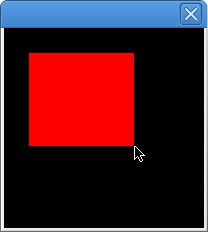
\includegraphics[width=0.3\textwidth]{01.png}
&
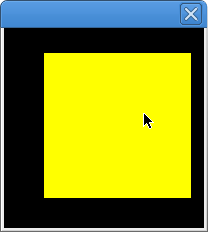
\includegraphics[width=0.3\textwidth]{02.png}
\end{tabular}
\begin{hscode}\SaveRestoreHook
\column{B}{@{}>{\hspre}l<{\hspost}@{}}%
\column{9}{@{}>{\hspre}l<{\hspost}@{}}%
\column{11}{@{}>{\hspre}l<{\hspost}@{}}%
\column{15}{@{}>{\hspre}l<{\hspost}@{}}%
\column{E}{@{}>{\hspre}l<{\hspost}@{}}%
\>[B]{}\mathbf{type}\;\Conid{Box}\mathrel{=}(\Conid{Rect},\Conid{Color}){}\<[E]%
\\
\>[B]{}\Varid{define}{}\<[15]%
\>[15]{}\mathbin{::}\Conid{S}\;\Conid{GUIEv}\;\Conid{Box}\;\Conid{Rect}{}\<[E]%
\\
\>[B]{}\Varid{chooseColor}{}\<[15]%
\>[15]{}\mathbin{::}\Conid{Rect}\to \Conid{S}\;\Conid{GUIEvBox}\;\Conid{Color}{}\<[E]%
\\
\>[B]{}\Varid{clickOn}{}\<[15]%
\>[15]{}\mathbin{::}\Conid{Rect}\to \Conid{R}\;\Conid{GUIEv}\;(){}\<[E]%
\\
\>[B]{}\Varid{box}\mathbin{::}{}\<[9]%
\>[9]{}\Conid{S}\;\Conid{GUIEv}\;\Conid{Box}\;(){}\<[E]%
\\
\>[B]{}\Varid{box}\mathrel{=}\mathbf{do}\;{}\<[11]%
\>[11]{}\Varid{r}\leftarrow \Varid{define}{}\<[E]%
\\
\>[11]{}\Varid{chooseColor}\;\Varid{r}{}\<[E]%
\\
\>[11]{}\Varid{waitFor}\;(\Varid{clickOn}\;\Varid{r}){}\<[E]%
\ColumnHook
\end{hscode}\resethooks
\end{frame}


\begin{frame}{Another Signal computations example}
\begin{hscode}\SaveRestoreHook
\column{B}{@{}>{\hspre}l<{\hspost}@{}}%
\column{11}{@{}>{\hspre}l<{\hspost}@{}}%
\column{E}{@{}>{\hspre}l<{\hspost}@{}}%
\>[B]{}\mathbf{newtype}\;\Conid{S}\;\Varid{ev}\;\Varid{f}\;\Varid{r}\mathrel{=}\dots{}\<[E]%
\\
\>[B]{}\mathbf{instance}\;\Conid{Monad}\;(\Conid{S}\;\Varid{ev}\;\Varid{f})\;\mathbf{where}\dots{}\<[E]%
\\
\>[B]{}\Varid{waitFor}{}\<[11]%
\>[11]{}\mathbin{::}\Conid{R}\;\Varid{ev}\;\Varid{r}\to \Conid{S}\;\Varid{ev}\;\Varid{f}\;\Varid{r}{}\<[E]%
\\
\>[B]{}\Varid{emit}{}\<[11]%
\>[11]{}\mathbin{::}\Varid{f}\to \Conid{S}\;\Varid{ev}\;\Varid{f}\;(){}\<[E]%
\ColumnHook
\end{hscode}\resethooks

Example: Cycle trough colors until right click 
\begin{hscode}\SaveRestoreHook
\column{B}{@{}>{\hspre}l<{\hspost}@{}}%
\column{4}{@{}>{\hspre}l<{\hspost}@{}}%
\column{6}{@{}>{\hspre}l<{\hspost}@{}}%
\column{10}{@{}>{\hspre}l<{\hspost}@{}}%
\column{E}{@{}>{\hspre}l<{\hspost}@{}}%
\>[B]{}\Varid{cycleColor}\mathbin{::}\Conid{S}\;\Conid{GUIEv}\;\Conid{Color}\;\Conid{Int}{}\<[E]%
\\
\>[B]{}\Varid{cycleColor}\mathrel{=}\Varid{cc}\;\Varid{colors}\;\mathrm{1}\;\mathbf{where}{}\<[E]%
\\
\>[B]{}\hsindent{4}{}\<[4]%
\>[4]{}\Varid{cc}\;(\Varid{h}\mathbin{:}\Varid{t})\;\Varid{i}\mathrel{=}{}\<[E]%
\\
\>[4]{}\hsindent{2}{}\<[6]%
\>[6]{}\mathbf{do}\;{}\<[10]%
\>[10]{}\Varid{emit}\;\Varid{h}{}\<[E]%
\\
\>[10]{}\Varid{r}\leftarrow \Varid{waitFor}\;(\Varid{middleClick}\mathbin{`\Varid{before}`}\Varid{rightClick}){}\<[E]%
\\
\>[10]{}\mathbf{if}\;\Varid{r}\;\mathbf{then}\;\Varid{cc}\;\Varid{t}\;(\Varid{i}\mathbin{+}\mathrm{1})\;\mathbf{else}\;\Varid{return}\;\Varid{i}{}\<[E]%
\ColumnHook
\end{hscode}\resethooks

\end{frame}

\begin{frame}{Dynamic lists}
\begin{center}
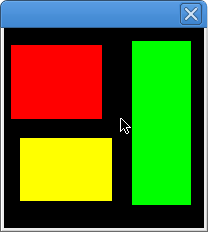
\includegraphics[width=0.3\textwidth]{05.png}
\end{center}


\begin{hscode}\SaveRestoreHook
\column{B}{@{}>{\hspre}l<{\hspost}@{}}%
\column{7}{@{}>{\hspre}l<{\hspost}@{}}%
\column{E}{@{}>{\hspre}l<{\hspost}@{}}%
\>[B]{}\Varid{boxes}\mathbin{::}\Conid{S}\;\Conid{GUIEv}\;[\mskip1.5mu \Conid{Box}\mskip1.5mu]\;(){}\<[E]%
\\
\>[B]{}\Varid{boxes}\mathrel{=}\Varid{rList}\;\Varid{box}{}\<[E]%
\\[\blanklineskip]%
\>[B]{}\Varid{rList}\mathbin{::}\Conid{S}\;\Varid{ef}\;\Varid{f}\;\Varid{a}\to \Conid{S}\;\Varid{ef}\;[\mskip1.5mu \Varid{f}\mskip1.5mu]\;(){}\<[E]%
\\
\>[B]{}\Varid{box}{}\<[7]%
\>[7]{}\mathbin{::}\Conid{S}\;\Conid{GUIEv}\;\Conid{Box}\;(){}\<[E]%
\ColumnHook
\end{hscode}\resethooks

\begin{itemize}
\item Start a new \ensuremath{\Varid{box}} computation, and when it starts, add it to the list and repeat
\item If a \ensuremath{\Varid{box}} computation ends remove it from the list
\end{itemize}
\end{frame}

\begin{frame}{Programmer interface summary}

\end{frame}

\section{Programmer interface comparison}
\begin{frame}{Comparison with Arrowized FRP}
Monadic FRP:
\begin{hscode}\SaveRestoreHook
\column{B}{@{}>{\hspre}l<{\hspost}@{}}%
\column{3}{@{}>{\hspre}l<{\hspost}@{}}%
\column{5}{@{}>{\hspre}l<{\hspost}@{}}%
\column{E}{@{}>{\hspre}l<{\hspost}@{}}%
\>[B]{}\Varid{cycleColor}\mathbin{::}\Conid{S}\;\Conid{GUIEv}\;\Conid{Color}\;\Conid{Int}{}\<[E]%
\\
\>[B]{}\Varid{cycleColor}\mathrel{=}\Varid{cc}\;\Varid{colors}\;\mathrm{1}\;\mathbf{where}{}\<[E]%
\\
\>[B]{}\hsindent{3}{}\<[3]%
\>[3]{}\Varid{cc}\;(\Varid{h}\mathbin{:}\Varid{t})\;\Varid{i}\mathrel{=}\mathbf{do}{}\<[E]%
\\
\>[3]{}\hsindent{2}{}\<[5]%
\>[5]{}\Varid{emit}\;\Varid{h}{}\<[E]%
\\
\>[3]{}\hsindent{2}{}\<[5]%
\>[5]{}\Varid{r}\leftarrow \Varid{waitFor}\;(\Varid{middleClick}\mathbin{`\Varid{before}`}\Varid{rightClick}){}\<[E]%
\\
\>[3]{}\hsindent{2}{}\<[5]%
\>[5]{}\mathbf{if}\;\Varid{r}\;\mathbf{then}\;\Varid{cc}\;\Varid{t}\;(\Varid{i}\mathbin{+}\mathrm{1})\;\mathbf{else}\;\Varid{return}\;\Varid{i}{}\<[E]%
\ColumnHook
\end{hscode}\resethooks
Arrowized FRP:
\begin{hscode}\SaveRestoreHook
\column{B}{@{}>{\hspre}l<{\hspost}@{}}%
\column{3}{@{}>{\hspre}l<{\hspost}@{}}%
\column{5}{@{}>{\hspre}l<{\hspost}@{}}%
\column{7}{@{}>{\hspre}l<{\hspost}@{}}%
\column{11}{@{}>{\hspre}l<{\hspost}@{}}%
\column{38}{@{}>{\hspre}l<{\hspost}@{}}%
\column{E}{@{}>{\hspre}l<{\hspost}@{}}%
\>[B]{}\Varid{cycleColor}\mathbin{::}\Conid{SF}\;\Conid{MouseDown}\;(\Conid{Color},\Conid{Event}\;\Conid{Int}){}\<[E]%
\\
\>[B]{}\Varid{cycleColor}\mathrel{=}\Varid{cc}\;\Varid{colors}\;\mathrm{1}\;\mathbf{where}{}\<[E]%
\\
\>[B]{}\hsindent{3}{}\<[3]%
\>[3]{}\Varid{cc}\;(\Varid{h}\mathbin{:}\Varid{t})\;\Varid{i}\mathrel{=}\Varid{switch}\;(\Varid{proc}\;\Varid{md}\to \mathbf{do}{}\<[E]%
\\
\>[3]{}\hsindent{4}{}\<[7]%
\>[7]{}\Varid{mc}{}\<[11]%
\>[11]{}\leftarrow \Varid{notYet}<\!\!\!<\!\!\!<\Varid{middleClick}{}\<[38]%
\>[38]{}\:-\!\!\!<\Varid{md}{}\<[E]%
\\
\>[3]{}\hsindent{4}{}\<[7]%
\>[7]{}\Varid{rc}{}\<[11]%
\>[11]{}\leftarrow \Varid{rightClick}{}\<[38]%
\>[38]{}\:-\!\!\!<\Varid{md}{}\<[E]%
\\
\>[3]{}\hsindent{4}{}\<[7]%
\>[7]{}\Varid{returnA}\:-\!\!\!<((\Varid{h},\Varid{tag}\;\Varid{rc}\;\Varid{i}),\Varid{mc}){}\<[E]%
\\
\>[3]{}\hsindent{2}{}\<[5]%
\>[5]{})(\lambda \anonymous \to \Varid{cc}\;\Varid{t}\;(\Varid{i}\mathbin{+}\mathrm{1})){}\<[E]%
\ColumnHook
\end{hscode}\resethooks

\end{frame}

\begin{frame}{Comparison with Arrowized FRP}
Monadic FRP:
\begin{hscode}\SaveRestoreHook
\column{B}{@{}>{\hspre}l<{\hspost}@{}}%
\column{E}{@{}>{\hspre}l<{\hspost}@{}}%
\>[B]{}\Varid{boxes}\mathbin{::}\Conid{S}\;[\mskip1.5mu \Conid{Box}\mskip1.5mu]\;(){}\<[E]%
\\
\>[B]{}\Varid{boxes}\mathrel{=}\Varid{dynList}\;(\Varid{spawn}\;\Varid{box}){}\<[E]%
\ColumnHook
\end{hscode}\resethooks
Arrowized FRP:
\begin{hscode}\SaveRestoreHook
\column{B}{@{}>{\hspre}l<{\hspost}@{}}%
\column{3}{@{}>{\hspre}l<{\hspost}@{}}%
\column{5}{@{}>{\hspre}l<{\hspost}@{}}%
\column{11}{@{}>{\hspre}l<{\hspost}@{}}%
\column{13}{@{}>{\hspre}l<{\hspost}@{}}%
\column{21}{@{}>{\hspre}l<{\hspost}@{}}%
\column{E}{@{}>{\hspre}l<{\hspost}@{}}%
\>[B]{}\mathbf{type}\;\Conid{BoxSF}{}\<[13]%
\>[13]{}\mathrel{=}\Conid{SF}\;\Conid{GUIIn}\;(\Conid{Box},\Conid{Event}\;()){}\<[E]%
\\[\blanklineskip]%
\>[B]{}\Varid{boxes}\mathbin{::}\Conid{SF}\;\Conid{GUIIn}\;[\mskip1.5mu \Conid{Box}\mskip1.5mu]{}\<[E]%
\\
\>[B]{}\Varid{boxes}\mathrel{=}\Varid{boxes'}\;[\mskip1.5mu \mskip1.5mu]>\!\!\!>\!\!\!>\Varid{arr}\;(\Varid{map}\;\Varid{fst})\;\mathbf{where}{}\<[E]%
\\
\>[B]{}\hsindent{3}{}\<[3]%
\>[3]{}\Varid{boxes'}\;\Varid{i}\mathrel{=}\Varid{pSwitchList}\;\Varid{i}{}\<[E]%
\\
\>[3]{}\hsindent{2}{}\<[5]%
\>[5]{}(\Varid{newBox}*\!\!*\!\!*\Varid{arr}\;\Varid{toEv}>\!\!\!>\!\!\!>\Varid{arr}\;\Varid{choose}>\!\!\!>\!\!\!>\Varid{notYet}){}\<[E]%
\\
\>[3]{}\hsindent{2}{}\<[5]%
\>[5]{}(\lambda \Varid{e}\;\Varid{l}\to \Varid{boxes'}\;(\Varid{mutateList}\;\Varid{e}\;\Varid{l})){}\<[E]%
\\
\>[B]{}\Varid{choose}\;(\Varid{a},\Varid{b})\mathrel{=}\Varid{merge}\;(\Varid{fmap}\;\Conid{Left}\;\Varid{a})\;(\Varid{fmap}\;\Conid{Right}\;\Varid{b}){}\<[E]%
\\
\>[B]{}\Varid{toEv}\;\Varid{l}\mathrel{=}{}\<[11]%
\>[11]{}\mathbf{let}\;\Varid{l'}\mathrel{=}\Varid{map}\;(\Varid{isNoEvent}\mathbin{\circ}\Varid{snd})\;\Varid{l}{}\<[E]%
\\
\>[11]{}\mathbf{in}\;\mathbf{if}\;\Varid{and}\;\Varid{l'}\;\mathbf{then}\;\Conid{NoEvent}\;\mathbf{else}\;\Conid{Event}\;\Varid{l'}{}\<[E]%
\\
\>[B]{}\Varid{mutate}\;\Varid{l}\;(\Conid{Left}\;\Varid{b}){}\<[21]%
\>[21]{}\mathrel{=}\Varid{b}\mathbin{:}\Varid{l}{}\<[E]%
\\
\>[B]{}\Varid{mutate}\;\Varid{l}\;(\Conid{Right}\;\Varid{l'})\mathrel{=}\Varid{map}\;\Varid{fst}\;(\Varid{filter}\;\Varid{snd}\;(\Varid{zip}\;\Varid{l}\;\Varid{l'})){}\<[E]%
\ColumnHook
\end{hscode}\resethooks
\end{frame}

\begin{frame}{Advantages \& disadvantages of Monadic FRP API}
Advantages: 
\begin{itemize}
\item Implicit routing
\item Sequencing phases is easier \& more intuitive.
\item Easier dynamic lists 
\end{itemize}
Disadvantages:
\begin{itemize}
\item Currently no reactive-level recursion
\item Explicit memoization needed for reactive-level sharing
\end{itemize}
\end{frame}

\section{Evaluation model}
\begin{frame}{Evaluation model: context}
Other FRP evaluation models either:
\begin{itemize}
\item Re-evaluate the whole expression after each event
\item Use side-effects to prevent redundant re-evalutions
\end{itemize}

Monadic FRP has the first \emph{purely functional} evaluation model that prevents redundant re-evaluations.

\end{frame}

\begin{frame}{Idea}
We do not know if a reactive computation an event will have any effect on a reactive computation:
\begin{hscode}\SaveRestoreHook
\column{B}{@{}>{\hspre}l<{\hspost}@{}}%
\column{14}{@{}>{\hspre}c<{\hspost}@{}}%
\column{14E}{@{}l@{}}%
\column{18}{@{}>{\hspre}l<{\hspost}@{}}%
\column{E}{@{}>{\hspre}l<{\hspost}@{}}%
\>[B]{}\mathbf{data}\;\Conid{R}\;\Varid{ev}\;\Varid{a}{}\<[14]%
\>[14]{}\approx{}\<[14E]%
\>[18]{}\Conid{Await}\;(\Varid{ev}\to \Conid{React}\;\Varid{a}){}\<[E]%
\\
\>[14]{}\mid {}\<[14E]%
\>[18]{}\Conid{Done}\;\Varid{a}{}\<[E]%
\ColumnHook
\end{hscode}\resethooks
\pause
Communicate which events a reactive computation is intrested in:
\begin{hscode}\SaveRestoreHook
\column{B}{@{}>{\hspre}l<{\hspost}@{}}%
\column{14}{@{}>{\hspre}c<{\hspost}@{}}%
\column{14E}{@{}l@{}}%
\column{18}{@{}>{\hspre}l<{\hspost}@{}}%
\column{E}{@{}>{\hspre}l<{\hspost}@{}}%
\>[B]{}\mathbf{data}\;\Conid{R}\;\Varid{ev}\;\Varid{a}{}\<[14]%
\>[14]{}\approx{}\<[14E]%
\>[18]{}\Conid{Await}\;(\Conid{Requests}\;\Varid{ev})\;(\Varid{ev}\to \Conid{React}\;\Varid{a}){}\<[E]%
\\
\>[14]{}\mid {}\<[14E]%
\>[18]{}\Conid{Done}\;\Varid{a}{}\<[E]%
\ColumnHook
\end{hscode}\resethooks
No reevalution: Only call a continuation if it is intrested in the occured event

\end{frame}

\begin{frame}{Effects on basic combinators}

\begin{itemize}
\item \ensuremath{\Varid{a}\bind \Varid{b}} requests the same events as \ensuremath{\Varid{a}}
\item \ensuremath{\Varid{first}\;\Varid{a}\;\Varid{b}} requests the union of the requests of \ensuremath{\Varid{a}} and \ensuremath{\Varid{b}} 
\end{itemize}
All other (Signal computation) combinators are expressed in terms of \ensuremath{\bind } and \ensuremath{\Varid{first}}

\end{frame}

\centering
\tikzstyle{bag} = [rectangle,text centered,draw=black,semithick,solid]
\tikzstyle{interpret} = [rectangle, rounded corners,text centered,draw=black,semithick]
 \tikzstyle{every node}=[font=\small]

\begin{frame}{Example evaluation}

\begin{tikzpicture}[grow=down, level distance=60pt]
[-]

\node[bag, name=root] {\ensuremath{\Varid{first}}}
  [sibling distance=4.5cm]
  child {node[bag] {\ensuremath{\Varid{first}}}[sibling distance=2cm]
    child {node[bag] {\ensuremath{\Varid{mouseMove}}}
       edge from parent[<-]
       node[xshift=-15pt,midway,fill=white,color=white,text=black]{$\{\mathit{MouseMove}\}$}
    }
    child {node[bag] {\ensuremath{\Varid{mouseUp}}}
       edge from parent[<-]
       node[xshift=+15pt,midway,fill=white,color=white,text=black]{$\{\mathit{MouseUp}\}$}
    }
       edge from parent[<-]
       node[xshift=-15pt,midway,fill=white,color=white,text=black]{$\{\mathit{MouseMove},\mathit{MouseUp}\}$}
       %node[left]{$\{\mathit{MouseMove},$ \\ $\mathit{MouseUp}\}$}
  }
   child {node[bag] {\ensuremath{\sequ }}  [sibling distance=2.4cm]
child {node[bag] {\ensuremath{\Varid{mouseDown}}}
       edge from parent[<-]
       node[midway,fill=white,color=white,text=black]{$\{\mathit{MouseDown}\}$}
    }
    child {node[bag] {\ensuremath{\Varid{deltaTime}}}
       edge from parent[-]
    }
       edge from parent[<-]
       node[xshift=+15pt,midway,fill=white,color=white,text=black]{$\{\mathit{MouseDown}\}$}
  }
 
 ;
\node[interpret,above of=root,yshift=+20pt,name=inter,text width=3cm] {Reactive Interpreter};
\draw [->] (root) --  (inter) node[midway,fill=white,color=white,text=black]{$\{\mathit{MouseMove},\mathit{MouseUp}, \mathit{MouseDown}\}$};
\end{tikzpicture} 
\begin{hscode}\SaveRestoreHook
\column{B}{@{}>{\hspre}l<{\hspost}@{}}%
\column{E}{@{}>{\hspre}l<{\hspost}@{}}%
\>[B]{}\Varid{first}\;(\Varid{first}\;\Varid{mouseMove}\;\Varid{mouseUp})\;(\Varid{mouseDown}\sequ \Varid{deltaTime}){}\<[E]%
\ColumnHook
\end{hscode}\resethooks
\end{frame}


\begin{frame}{Example evaluation}

\begin{tikzpicture}[grow=down, level distance=60pt]
[-]

\node[bag, name=root] {\ensuremath{\Varid{first}}}
  [sibling distance=4.5cm]
  child {node[bag] {\ensuremath{\Varid{first}}}[sibling distance=2cm]
    child {node[bag] {\ensuremath{\Varid{mouseMove}}}
       edge from parent[-,dashed]
       node[xshift=-15pt,midway,fill=white,color=white,text=black]{$\{\mathit{MouseMove}\}$}
    }
    child {node[bag] {\ensuremath{\Varid{mouseUp}}}
       edge from parent[-,dashed]
       node[xshift=+15pt,midway,fill=white,color=white,text=black]{$\{\mathit{MouseUp}\}$}
    }
       edge from parent[-,dashed]
       node[xshift=-15pt,midway,fill=white,color=white,text=black]{$\{\mathit{MouseMove},\mathit{MouseUp}\}$}
       %node[left]{$\{\mathit{MouseMove},$ \\ $\mathit{MouseUp}\}$}
  }
   child {node[bag] {\ensuremath{\sequ }}  [sibling distance=2.4cm]
child {node[bag] {\ensuremath{\Varid{mouseDown}}}
       edge from parent[->,very thick]
       node[midway,fill=white,color=white,text=black]{$\{\mathit{MouseDown}\}$}
    }
    child {node[bag] {\ensuremath{\Varid{deltaTime}}}
       edge from parent[-,dashed]
    }
       edge from parent[->,very thick]
       node[xshift=+15pt,midway,fill=white,color=white,text=black]{$\{\mathit{MouseDown}\}$}
  }
 
 ;
\node[interpret,above of=root,yshift=+20pt,name=inter,text width=3cm] {Reactive Interpreter};
\draw [<-,very thick] (root) --  (inter) node[midway,fill=white,color=white,text=black]{Observed: $\mathit{MouseDown}$};

\end{tikzpicture} 
\begin{hscode}\SaveRestoreHook
\column{B}{@{}>{\hspre}l<{\hspost}@{}}%
\column{E}{@{}>{\hspre}l<{\hspost}@{}}%
\>[B]{}\Varid{first}\;(\Varid{first}\;\Varid{mouseMove}\;\Varid{mouseUp})\;(\Varid{mouseDown}\sequ \Varid{deltaTime}){}\<[E]%
\ColumnHook
\end{hscode}\resethooks
\end{frame}

\begin{frame}{Example evaluation}

\begin{tikzpicture}[grow=down, level distance=60pt]
[-]

\node[bag, name=root] {\ensuremath{\Varid{first}}}
  [sibling distance=4.5cm]
  child {node[bag] {\ensuremath{\Varid{first}}}[sibling distance=2cm]
    child {node[bag] {\ensuremath{\Varid{mouseMove}}}
       edge from parent[<-]
       node[xshift=-15pt,midway,fill=white,color=white,text=black]{$\{\mathit{MouseMove}\}$}
    }
    child {node[bag] {\ensuremath{\Varid{mouseUp}}}
       edge from parent[<-]
       node[xshift=+15pt,midway,fill=white,color=white,text=black]{$\{\mathit{MouseUp}\}$}
    }
       edge from parent[<-]
       node[xshift=-15pt,midway,fill=white,color=white,text=black]{$\{\mathit{MouseMove},\mathit{MouseUp}\}$}
       %node[left]{$\{\mathit{MouseMove},$ \\ $\mathit{MouseUp}\}$}
  }
   child {node[bag] {\ensuremath{\Varid{deltaTime}}}  [sibling distance=2.4cm]
       edge from parent[<-]
       node[xshift=+15pt,midway,fill=white,color=white,text=black]{$\{\mathit{DeltaTime}\}$}
  }
 
 ;
\node[interpret,above of=root,yshift=+20pt,name=inter,text width=3cm] {Reactive Interpreter};
\draw [->] (root) --  (inter) node[midway,fill=white,color=white,text=black]{$\{\mathit{MouseMove},\mathit{MouseUp}, \mathit{DeltaTime}\}$};
\end{tikzpicture} 
\begin{hscode}\SaveRestoreHook
\column{B}{@{}>{\hspre}l<{\hspost}@{}}%
\column{E}{@{}>{\hspre}l<{\hspost}@{}}%
\>[B]{}\Varid{first}\;(\Varid{first}\;\Varid{mouseMove}\;\Varid{mouseUp})\;\Varid{deltaTime}{}\<[E]%
\ColumnHook
\end{hscode}\resethooks
\end{frame}

\end{document}
